\section{Frozen phonons and linear response}\label{sec:5.4}

The dispersion of silicon in \cref{fig:5-si} came from sixteen calculations, each in the two-atom primitive cell, one for each inequivalent wavevector of a $6\times6\times6$ grid. The same force constants could have been obtained by moving atoms in a supercell of $6^3 = 216$ primitive cells, 432 atoms, and recording the forces. The cost of a density-functional calculation grows as the cube of the number of atoms $N_{\mathrm{at}}$ in the cell times the number of $\vect{k}$ points. A cell $n$ times larger needs $n$ times fewer $\vect{k}$ points for the same sampling, as long as more than one is left. Each self-consistent calculation of that supercell would therefore cost $216^3/216 = 216^2 \approx 5\times10^4$ times one of the primitive cell. The two routes measure the same thing, the second derivatives of the energy surface $E^{\mathrm{ad}}(u)$ of \cref{sec:5.1}, from finite differences of forces or from the linear response of the electrons to a displacement wave. The Sternheimer equation makes the linear-response route, DFPT, cheap, and Fourier interpolation turns a few dynamical matrices into the whole dispersion. Our account follows Baroni and coworkers~\cite{baroni2001phonons} and Giustino~\cite{giustino2017electron}.

\subsection{Frozen phonons}

The most direct way to get a force constant is to displace an atom and measure the forces on all the others. The force on the nucleus $(\vect{R},\kappa')$ along $\alpha$ when only the nucleus $(\vect{0},\kappa)$ is displaced by $h$ along $\beta$ is, by \cref{eq:5.2-expand} carried one order further,
\begin{equation*}
  F^\alpha_{\vect{R}\kappa'}(h) = -\Phi^{(2),\alpha\beta}_{\kappa'\kappa}(\vect{R},\vect{0})\,h - \tfrac12\Phi^{(3),\alpha\beta\beta}_{\kappa'\kappa\kappa}(\vect{R},\vect{0},\vect{0})\,h^2 - \tfrac16\Phi^{(4),\alpha\beta\beta\beta}_{\kappa'\kappa\kappa\kappa}(\vect{R},\vect{0},\vect{0},\vect{0})\,h^3 + O(h^4) ,
\end{equation*}
where $\Phi^{(3)}$ and $\Phi^{(4)}$ are the third and fourth derivatives of $E^{\mathrm{ad}}$ (\cref{sec:5.7}). The forces are the Hellmann--Feynman forces of \cref{eq:5.1-HF}, which a code returns at the cost of one self-consistent calculation. The quotient $-F/h$ has an error of first order in $h$, from the cubic term. Displacing by $+h$ and by $-h$ and taking the difference cancels all even powers of $h$:
\begin{equation}
  \Phi^{(2),\alpha\beta}_{\kappa'\kappa}(\vect{R},\vect{0}) = -\frac{F^\alpha_{\vect{R}\kappa'}(h) - F^\alpha_{\vect{R}\kappa'}(-h)}{2h} + O(h^2) .
  \label{eq:5.4-fd}
\end{equation}
This is the \emph{frozen-phonon} method in its finite-displacement form~\cite[Sect.~IV.B]{baroni2001phonons}. Because each calculation returns the force on every nucleus, one displacement gives a whole column of the force-constant matrix, $3N_{\mathrm{at}}$ numbers for a cell of $N_{\mathrm{at}}$ atoms; an energy alone would give one number. Symmetry reduces the work further. In silicon both atoms of the cell are equivalent under the space group, and the site symmetry $T_d$ contains the threefold rotation about $[111]$ that turns $x$ into $y$ and $z$. A single displacement of one atom along $x$, made with both signs, therefore fixes every force constant the supercell can hold. The step $h$ is a compromise: large enough that the force exceeds the numerical noise of the calculation, typically \SIrange{0.01}{0.03}{\angstrom}, and small enough that the $O(h^2)$ term of \cref{eq:5.4-fd}, set by $\Phi^{(4)}$, is negligible.

A displaced atom in a periodic calculation is not alone. A supercell built from $N_Q\times N_Q\times N_Q$ primitive cells repeats with the lattice of supercell translations $\vect{T}$, and moving the nucleus $(\vect{0},\kappa)$ moves all its images $(\vect{T},\kappa)$ with it. The force recorded on $(\vect{R},\kappa')$ is then the sum over images. With $\Phi^{(2)}(\vect{R},\vect{T}) = \Phi^{(2)}(\vect{R}-\vect{T},\vect{0})$ by translation invariance (\cref{sec:5.2}), the supercell measures
\begin{equation}
  \Phi^{\mathrm{SC},\alpha\beta}_{\kappa'\kappa}(\vect{R}) = \sum_{\vect{T}}\Phi^{(2),\alpha\beta}_{\kappa'\kappa}(\vect{R}+\vect{T},\vect{0}) ,
  \label{eq:5.4-alias}
\end{equation}
a sum of the true constant and its copies displaced by every supercell translation. The true $\Phi^{(2)}$ cannot be recovered from $\Phi^{\mathrm{SC}}$ in general, but the dynamical matrix can, at special wavevectors. Write each cell vector of \cref{eq:5.2-Ddyn} as $\vect{R} = \vect{R}_s + \vect{T}$, with $\vect{R}_s$ one of the $N_Q^3$ cells of the supercell. If $\ee^{\ii\vect{Q}\cdot\vect{T}} = 1$ for every $\vect{T}$, the phase depends only on $\vect{R}_s$, the sum over $\vect{T}$ acts on $\Phi^{(2)}$ alone, and
\begin{equation*}
  D^{\mathrm{dyn},\alpha\beta}_{\kappa\kappa'}(\vect{Q}) = \frac{1}{\sqrt{M_\kappa M_{\kappa'}}}\sum_{\vect{R}_s}\Phi^{\mathrm{SC},\alpha\beta}_{\kappa\kappa'}(\vect{R}_s)\,\ee^{\ii\vect{Q}\cdot\vect{R}_s}
\end{equation*}
holds exactly, with $\Phi^{\mathrm{SC}}_{\kappa\kappa'}(\vect{R}_s)$ read off the supercell with the roles of the two nuclei exchanged by pair symmetry. The wavevectors with $\ee^{\ii\vect{Q}\cdot\vect{T}} = 1$ are the $N_Q^3$ points of a uniform grid in the zone, the zone center among them. A frozen-phonon calculation in an $N_Q^3$ supercell therefore gives the exact phonons on an $N_Q^3$ grid of wavevectors and nothing more. At the zone center the primitive cell is the supercell. The zone-boundary point X of silicon, $\vect{Q} = (0,0,1)\,2\pi/a$, has $\ee^{\ii\vect{Q}\cdot\vect{R}} = -1$ for half of the cell vectors and needs a cell twice as large, as the doubled period of the folded chain in \cref{we:5-chain} already showed. Long wavelengths need large cells. Force constants of range $L$ need a supercell of side $\sim L$, with $N_{\mathrm{at}} \propto L^3$ atoms. By the rule of the opening paragraph each calculation then costs $\propto N_{\mathrm{at}}^3$ times the number of $\vect{k}$ points: $\propto L^6$ while the $\vect{k}$ grid can still be thinned, and $\propto L^9$ once a single $\vect{k}$ point suffices, the regime of the ninth-power scaling quoted by Baroni and coworkers~\cite[Sect.~IV.B]{baroni2001phonons} and worked out in \cref{app:E.4}. A dark-matter calculation needs the acoustic branches precisely near the zone center, where this route is most expensive.

The energy itself, rather than the force, yields a frequency in one stroke when the pattern of the displacement is fixed by symmetry. This is the original frozen-phonon method~\cite[Sect.~IV.B]{baroni2001phonons}: the atoms are displaced along a known normal mode, and the energy is fitted as a function of its amplitude. The zone-center optical mode of silicon is such a mode.

\begin{workedexample}{The optical frequency of silicon from a frozen phonon}\label{we:5-frozen}
At the zone center the two atoms of the cell move against each other, and by symmetry the polarization is fixed up to its direction. For a displacement along $[111]$, atom 1 moves by $-(u/2)\hat{\vect{n}}$ and atom 2 by $+(u/2)\hat{\vect{n}}$, with $\hat{\vect{n}} = (1,1,1)/\sqrt3$, so that the bond along $[111]$ changes its length by $u$. Every cell moves in the same way, and the primitive cell is the whole calculation. The energy per cell is $E^{\mathrm{ad}}_{\mathrm{cell}}(u) = \tfrac12\Phi_{\mathrm{opt}}u^2 + \tfrac16\Phi^{(3)}_{\mathrm{opt}}u^3 + \tfrac1{24}\Phi^{(4)}_{\mathrm{opt}}u^4 + \dots$, measured from the minimum. In the PBE calculation of \cref{fig:5-scales}, $E^{\mathrm{ad}}_{\mathrm{cell}} = \SI{5.943}{meV}$ at $u = +\SI{0.03}{\angstrom}$ and \SI{6.316}{meV} at $u = -\SI{0.03}{\angstrom}$. The bond resists compression more than stretching.

From a single energy, $2E^{\mathrm{ad}}_{\mathrm{cell}}(u)/u^2 = \Phi_{\mathrm{opt}} + \Phi^{(3)}_{\mathrm{opt}}u/3 + \dots$, we find $\Phi_{\mathrm{opt}} = \SI{13.21}{eV.\angstrom^{-2}}$ from the stretched bond and \SI{14.04}{eV.\angstrom^{-2}} from the compressed one. The spread is the cubic term: half the difference, $\SI{0.415}{eV.\angstrom^{-2}} = |\Phi^{(3)}_{\mathrm{opt}}|u/3$, puts $\Phi^{(3)}_{\mathrm{opt}}$ at \SI{-41.5}{eV.\angstrom^{-3}}, the value of \cref{sec:5.1}. The symmetric combination removes it,
\begin{equation*}
  \frac{E^{\mathrm{ad}}_{\mathrm{cell}}(u) + E^{\mathrm{ad}}_{\mathrm{cell}}(-u) - 2E^{\mathrm{ad}}_{\mathrm{cell}}(0)}{u^2} = \Phi_{\mathrm{opt}} + \frac{\Phi^{(4)}_{\mathrm{opt}}u^2}{12} + \dots = \SI{13.62}{eV.\angstrom^{-2}} ,
\end{equation*}
and the same combination at $u = \SI{0.06}{\angstrom}$ is \SI{13.64}{eV.\angstrom^{-2}}. The two symmetric estimates differ by \SI{0.02}{eV.\angstrom^{-2}}, within the precision of the computed energies, so the quartic term has to come from a fit to the whole curve. Polynomial fits to all the computed energies and forces, over ranges of $|u|$ from \SIrange{0.1}{0.3}{\angstrom}, put the quartic constant $\Phi^{(4)}_{\mathrm{opt}}$ at \SIrange{35}{42}{eV.\angstrom^{-4}}, about \SI{40}{eV.\angstrom^{-4}}, so the quartic correction $\Phi^{(4)}_{\mathrm{opt}}u^2/12$ is \SI{0.003}{eV.\angstrom^{-2}} at \SI{0.03}{\angstrom}, \SI{0.02}{\percent}. The coordinate $u$ carries the reduced mass $M_\kappa/2$, since each atom moves by $u/2$ and the kinetic energy is $\tfrac12(M_\kappa/2)\dot u^2$. With $M_\kappa = \SI{28.0855}{u}$,
\begin{equation*}
  \omega_{\mathrm{opt}} = \Bigl(\frac{2\Phi_{\mathrm{opt}}}{M_\kappa}\Bigr)^{1/2} = \SI{63.68}{meV} .
\end{equation*}
The central difference of the Hellmann--Feynman forces, \cref{eq:5.4-fd} applied to the coordinate $u$, yields \SI{13.63}{eV.\angstrom^{-2}} and \SI{63.71}{meV} from the same two calculations. DFPT at the same settings, the $4^3$ calculation of \cref{fig:5-scales}(b), finds \SI{63.7}{meV}, and the calculation of \cref{fig:5-si}, with a higher cutoff and a finer grid, \SI{63.69}{meV}. Neutron scattering finds \SI{64.1}{meV}~\cite{nilsson1972study}, \SI{0.6}{\percent} higher, a difference set by the functional and the static lattice, not by the method. The one-sided estimates, by contrast, miss by \SI{1.5}{\percent} at the smallest step and by \SI{3}{\percent} at \SI{0.06}{\angstrom}. A finite-difference force constant is accurate only when it is symmetric.
\end{workedexample}

\subsection{Force constants as a density response}

A second derivative of the energy needs only the first-order change of the electron density. Differentiate the Hellmann--Feynman force \cref{eq:5.1-HF} once more. Its electrostatic form contains the nuclear positions in two places, the electron--nucleus potential and the nucleus--nucleus repulsion, and the electron density, which also changes when a nucleus moves. In a Kohn--Sham calculation the electron--nucleus term is the external potential $V_{\mathrm{ext}}(\vect{r})$ of the electrons, the potential $U_1$ of \cref{eq:3.4-KS} and the operator $V_{eN}$ of \cref{eq:5.1-H}. Writing $E^{\mathrm{ad}} = E_{NN} + E_{\mathrm{el}}$, with $E_{NN}$ the repulsion of the nuclei and $\partial E_{\mathrm{el}}/\partial u_i = \int\dd^3r\,\nd(\vect{r})\,\partial V_{\mathrm{ext}}(\vect{r})/\partial u_i$ by the theorem, for any two displacement coordinates $u_i, u_j$~\cite[Eq.~(10)]{baroni2001phonons},
\begin{equation}
  \frac{\partial^2E^{\mathrm{ad}}}{\partial u_i\,\partial u_j}
  = \int\dd^3r\,\frac{\partial\nd(\vect{r})}{\partial u_j}\,\frac{\partial V_{\mathrm{ext}}(\vect{r})}{\partial u_i}
  + \int\dd^3r\,\nd(\vect{r})\,\frac{\partial^2V_{\mathrm{ext}}(\vect{r})}{\partial u_i\,\partial u_j}
  + \frac{\partial^2E_{NN}}{\partial u_i\,\partial u_j} .
  \label{eq:5.4-hess}
\end{equation}
The terms with $\nd$ and with $E_{NN}$ need only the ground state: the density at equilibrium and the positions of the nuclei, whose repulsion is an Ewald sum. The term with $\partial\nd/\partial u_j$ needs the change of the density to first order in a displacement, and nothing else. With a nonlocal pseudopotential (\cref{sec:3.5}) the integrals of $\nd$ against derivatives of $V_{\mathrm{ext}}$ become sums $2\sum_v\langle\psi_v|\partial V_{\mathrm{ext}}|\psi_v\rangle$ over occupied states, and the structure is unchanged.

A crystal is perturbed one wavevector at a time. Let the nuclei of species $\kappa$ move along $\alpha$ in a wave, $u^\beta_{\vect{R}\kappa'} = \delta_{\kappa\kappa'}\delta_{\alpha\beta}\,\lambda\,\ee^{\ii\vect{Q}\cdot\vect{R}}$. The derivative with respect to its amplitude is
\begin{equation*}
  \partial_{\kappa\alpha,\vect{Q}} = \sum_{\vect{R}}\ee^{\ii\vect{Q}\cdot\vect{R}}\,\frac{\partial}{\partial u^\alpha_{\vect{R}\kappa}} .
\end{equation*}
Applied to the bare potential, with $v_\kappa$ the potential of one nucleus (or pseudo-ion) of species $\kappa$, it yields $\partial_{\kappa\alpha,\vect{Q}}V_{\mathrm{ext}}(\vect{r}) = -\sum_{\vect{R}}\ee^{\ii\vect{Q}\cdot\vect{R}}\,\partial_\alpha v_\kappa(\vect{r} - \vect{R} - \vect{\tau}_\kappa)$, which is a lattice-periodic function times $\ee^{\ii\vect{Q}\cdot\vect{r}}$. The double sum $\sum_{\vect{R}\vect{R}'}\ee^{-\ii\vect{Q}\cdot\vect{R}}\ee^{\ii\vect{Q}\cdot\vect{R}'}\Phi^{(2)}(\vect{R},\vect{R}')$ collapses by translation invariance to $N\sum_{\vect{R}}\Phi^{(2)}(\vect{0},\vect{R})\,\ee^{\ii\vect{Q}\cdot\vect{R}}$, so the dynamical matrix \cref{eq:5.2-Ddyn} is a second derivative with respect to two such waves~\cite[Eq.~(82)]{baroni2001phonons},
\begin{equation}
  D^{\mathrm{dyn},\alpha\beta}_{\kappa\kappa'}(\vect{Q}) = \frac{1}{N\sqrt{M_\kappa M_{\kappa'}}}\,\partial_{\kappa\alpha,-\vect{Q}}\,\partial_{\kappa'\beta,\vect{Q}}\,E^{\mathrm{ad}} .
  \label{eq:5.4-Dwave}
\end{equation}
Inserted in \cref{eq:5.4-hess}, its electronic part contains the integral of $[\partial_{\kappa\alpha,\vect{Q}}V_{\mathrm{ext}}]^*\,\partial_{\kappa'\beta,\vect{Q}}\nd$ over the crystal~\cite[Eq.~(86)]{baroni2001phonons}, with $[\partial_{\vect{Q}}V]^* = \partial_{-\vect{Q}}V$ since the potential is real. The density response to the wave at $\vect{Q}$ carries the same crystal momentum: the perturbed crystal is invariant under a lattice translation combined with the phase $\ee^{\ii\vect{Q}\cdot\vect{R}}$, and so is its first-order density. Different $\vect{Q}$ decouple, and each is a problem in the primitive cell.

The density response is the static bubble of \cref{sec:4.6}. Kohn--Sham electrons move in $V_{\mathrm{KS}}$, and a change of it changes their density by $\delta\nd = R^0\,\delta V_{\mathrm{KS}}$, with $R^0$ the independent-particle response \cref{eq:4.6-R0} at $\omega = 0$. The potential itself responds to the density through the Hartree and exchange--correlation terms,
\begin{equation}
  \partial_{\kappa\alpha,\vect{Q}}V_{\mathrm{KS}}(\vect{r}) = \partial_{\kappa\alpha,\vect{Q}}V_{\mathrm{ext}}(\vect{r}) + \int\dd^3r'\,\bigl[v_{\mathrm{C}}(\vect{r}-\vect{r}') + f_{\mathrm{xc}}(\vect{r},\vect{r}')\bigr]\,\partial_{\kappa\alpha,\vect{Q}}\nd(\vect{r}') ,
  \label{eq:5.4-dV}
\end{equation}
where $f_{\mathrm{xc}}$ is the kernel \cref{eq:4.6-fxc} in its static form, the second functional derivative $\delta^2E_{\mathrm{xc}}/\delta\nd(\vect{r})\delta\nd(\vect{r}')$ of the ground-state functional~\cite[Eqs.~(42)--(46)]{giustino2017electron}. With $f_{\mathrm{Hxc}} = v_{\mathrm{C}} + f_{\mathrm{xc}}$, solving $\delta\nd = R^0(\delta V_{\mathrm{ext}} + f_{\mathrm{Hxc}}\delta\nd)$ for $\delta\nd$ yields $\delta\nd = R\,\delta V_{\mathrm{ext}}$, with $R = R^0 + R^0f_{\mathrm{Hxc}}R$ the Dyson equation \cref{eq:4.6-tddft} at zero frequency. Inserting $\partial\nd = R\,\partial V_{\mathrm{ext}}$ into the first term of \cref{eq:5.4-hess}, the electronic force constant is
\begin{equation*}
  \begin{split}
  N\sqrt{M_\kappa M_{\kappa'}}\,D^{\mathrm{dyn,el},\alpha\beta}_{\kappa\kappa'}(\vect{Q})
  &= \iint\dd^3r\,\dd^3r'\,\bigl[\partial_{\kappa\alpha,\vect{Q}}V_{\mathrm{ext}}(\vect{r})\bigr]^*R(\vect{r},\vect{r}';\omega = 0)\,\partial_{\kappa'\beta,\vect{Q}}V_{\mathrm{ext}}(\vect{r}') \\
  &\quad + \int\dd^3r\,\nd(\vect{r})\,\partial_{\kappa\alpha,-\vect{Q}}\partial_{\kappa'\beta,\vect{Q}}V_{\mathrm{ext}}(\vect{r}) ,
  \end{split}
\end{equation*}
the microscopic theory of force constants of Pick, Cohen and Martin~\cite{pick1970microscopic}. The bare nuclei and the rigid ground-state density give a stiff lattice; the static response $R$ is negative, since electrons move away from where their potential energy rises, and the electrons that flow to screen the displaced nuclei soften it. In a metal the screening is strong enough at long wavelength to turn the bare ionic plasma frequency into a sound wave. Within density-functional theory the static kernel is exactly $\delta^2E_{\mathrm{xc}}/\delta\nd\delta\nd$, so a DFPT phonon contains the full static electronic response of the functional, and its error is the error of the functional (\cref{app:E.4}). And since the electrons are relaxed at every frozen configuration, the adiabatic phonon frequency already includes the static part of the electron--phonon self-energy; \cref{app:D.17} uses this to avoid counting it twice.

\subsection{The Sternheimer equation}

The bubble \cref{eq:4.6-R0} is a sum over pairs of occupied and empty states, and a converged sum over empty states is expensive. DFPT avoids it. Start from the change of one occupied Kohn--Sham state. Linearizing $(H_{\mathrm{KS}} - \varepsilon_v)\psi_v = 0$ leads to~\cite[Eq.~(25)]{baroni2001phonons}
\begin{equation}
  (H_{\mathrm{KS}} - \varepsilon_v)\,|\delta\psi_v\rangle = -(\delta V_{\mathrm{KS}} - \delta\varepsilon_v)\,|\psi_v\rangle , \qquad \delta\varepsilon_v = \langle\psi_v|\delta V_{\mathrm{KS}}|\psi_v\rangle .
  \label{eq:5.4-lin}
\end{equation}
Solved by expanding in eigenstates it is ordinary first-order perturbation theory, $\delta\psi_v = \sum_{m\neq v}\psi_m\langle\psi_m|\delta V_{\mathrm{KS}}|\psi_v\rangle/(\varepsilon_v - \varepsilon_m)$. In the density, $\delta\nd = 2\sum_v(\psi_v^*\delta\psi_v + \psi_v\delta\psi_v^*)$ with the factor two for spin, the terms in which $m$ is another occupied state $v'$ cancel. The pair $(v,v')$ contributes $\psi_v^*\psi_{v'}\langle\psi_{v'}|\delta V_{\mathrm{KS}}|\psi_v\rangle/(\varepsilon_v - \varepsilon_{v'})$; the complex conjugate of the pair $(v',v)$ has the same numerator, since $\delta V_{\mathrm{KS}}$ is Hermitian, and the opposite denominator. A rotation among occupied states does not change the density, and only the component of $\delta\psi_v$ in the empty manifold matters~\cite[Eq.~(29)]{baroni2001phonons}. Call it $\op{P}^{\mathrm{c}}\delta\psi_v = \sum_c\psi_c\langle\psi_c|\delta V_{\mathrm{KS}}|\psi_v\rangle/(\varepsilon_v - \varepsilon_c)$, with $\op{P}^{\mathrm{c}} = 1 - \op{P}^{\mathrm{occ}}$ the projector on the empty states. Acting on it with $H_{\mathrm{KS}} - \varepsilon_v$ turns each denominator into $-1$:
\begin{equation*}
  (H_{\mathrm{KS}} - \varepsilon_v)\,\op{P}^{\mathrm{c}}|\delta\psi_v\rangle = -\sum_c|\psi_c\rangle\langle\psi_c|\delta V_{\mathrm{KS}}|\psi_v\rangle = -\op{P}^{\mathrm{c}}\,\delta V_{\mathrm{KS}}\,|\psi_v\rangle .
\end{equation*}
This is a linear equation for $\op{P}^{\mathrm{c}}\delta\psi_v$ whose right-hand side contains only the occupied state $\psi_v$. The empty states have disappeared, and so has $\delta\varepsilon_v$, which multiplies $\psi_v$ and is removed by the projector. The operator $H_{\mathrm{KS}} - \varepsilon_v$ is positive on the empty manifold of an insulator, where every eigenvalue exceeds $\varepsilon_v$, but singular or negative on the occupied one. Adding $a_{\mathrm{sh}}\op{P}^{\mathrm{occ}}$ changes nothing for a solution that lies in the empty manifold, and with $a_{\mathrm{sh}}$ larger than the valence bandwidth every eigenvalue $\varepsilon_{v'} + a_{\mathrm{sh}} - \varepsilon_v$ on the occupied manifold becomes positive too. The operator is then positive definite, and the equation can be solved by conjugate gradients with the cost of a few applications of $H_{\mathrm{KS}}$~\cite[Eq.~(30)]{baroni2001phonons}.

For a displacement wave the bookkeeping is in crystal momentum. The perturbation $\partial_{\kappa\alpha,\vect{Q}}V_{\mathrm{KS}}$ carries $\vect{Q}$, so its matrix element between $\psi_{v\vect{k}}$ and a state of crystal momentum $\vect{k}'$ vanishes unless $\vect{k}' = \vect{k} + \vect{Q}$ (\cref{sec:3.2}). The change of $\psi_{v\vect{k}}$ lives at $\vect{k} + \vect{Q}$, the projector is the one on the occupied states at $\vect{k}+\vect{Q}$, and $\delta\varepsilon_{v\vect{k}}$ vanishes unless $\vect{Q} = 0$, where the projector removes it.
\begin{keyresult}[Sternheimer equation of density-functional perturbation theory]
For each occupied state $\psi_{v\vect{k}}$ and each perturbation $(\kappa,\alpha,\vect{Q})$, the change $|\partial\psi_{v\vect{k}}\rangle$, of crystal momentum $\vect{k}+\vect{Q}$ and orthogonal to the occupied states, solves
\begin{equation}
  \bigl(H_{\mathrm{KS}} + a_{\mathrm{sh}}\op{P}^{\mathrm{occ}}_{\vect{k}+\vect{Q}} - \varepsilon_{v\vect{k}}\bigr)\,|\partial\psi_{v\vect{k}}\rangle
  = -\bigl(1 - \op{P}^{\mathrm{occ}}_{\vect{k}+\vect{Q}}\bigr)\,\partial_{\kappa\alpha,\vect{Q}}V_{\mathrm{KS}}\,|\psi_{v\vect{k}}\rangle ,
  \label{eq:5.4-sth}
\end{equation}
with $\op{P}^{\mathrm{occ}}_{\vect{k}+\vect{Q}} = \sum_{v'}|\psi_{v',\vect{k}+\vect{Q}}\rangle\langle\psi_{v',\vect{k}+\vect{Q}}|$ and $a_{\mathrm{sh}}$ larger than the valence bandwidth. The first-order density is
\begin{equation}
  \partial_{\kappa\alpha,\vect{Q}}\nd(\vect{r}) = 4\sum_{v\vect{k}}\psi^*_{v\vect{k}}(\vect{r})\,\partial\psi_{v\vect{k}}(\vect{r}) ,
  \label{eq:5.4-dn}
\end{equation}
and \cref{eq:5.4-dV,eq:5.4-sth,eq:5.4-dn} are solved to self-consistency.
\end{keyresult}
\Cref{eq:5.4-sth} is the equation of Baroni and coworkers~\cite[Eq.~(31)]{baroni2001phonons} and of Giustino~\cite[Eq.~(48)]{giustino2017electron}. The factor four in \cref{eq:5.4-dn} is two for spin and two from time reversal: the term $\psi_{v\vect{k}}\,(\partial_{-\vect{Q}}\psi_{v\vect{k}})^*$ of the density equals $\psi^*_{v,-\vect{k}}\,\partial_{\vect{Q}}\psi_{v,-\vect{k}}$ and doubles the sum over $\vect{k}$~\cite[Eq.~(35)]{baroni2001phonons}. Writing $\partial\psi_{v\vect{k}} = \ee^{\ii(\vect{k}+\vect{Q})\cdot\vect{r}}\,\partial u_{v\vect{k}}$ turns every quantity into a lattice-periodic function, and the calculation runs in the primitive cell at any $\vect{Q}$, commensurate or not, with a cost per perturbation comparable to that of the ground state.

The equation is old. Sternheimer used it in 1954 to compute the polarizabilities of ions without summing over excited states~\cite{sternheimer1954electronic}. In solids its self-consistent form, with the projector that makes it well posed, is due to Baroni, Giannozzi and Testa~\cite{baroni1987green} and to Giannozzi and coworkers, who computed the full dispersion of silicon and other semiconductors with it~\cite{giannozzi1991ab}. The self-consistency loop has the structure of a ground-state calculation: \cref{eq:5.4-sth} yields $\partial\psi$ for a trial potential, \cref{eq:5.4-dn} the density, \cref{eq:5.4-dV} a new potential. The loop starts from the bare $\partial V_{\mathrm{ext}}$ and converges to the screened $\partial V_{\mathrm{KS}}$, which is also the electron--phonon vertex of \cref{sec:6.2}. \Cref{app:E.4} describes what a run returns, its convergence parameters and its cost.

\subsection{The \texorpdfstring{$2n+1$}{2n+1} theorem}

The Hellmann--Feynman theorem gets a first derivative of the energy from the unperturbed state alone, and \cref{eq:5.4-hess} gets a second derivative from the first-order density. Both are the lowest cases of one statement. Let a perturbation of strength $\lambda$ change the energy functional to $E[\psi;\lambda]$, where $\psi$ stands for all the occupied orbitals, and let $\psi(\lambda)$ be its minimum, so that the ground-state energy is $E_0(\lambda) = E[\psi(\lambda);\lambda]$. Expand $\psi(\lambda) = \psi^{(0)} + \lambda\psi^{(1)} + \lambda^2\psi^{(2)} + \dots$ and $E_0(\lambda) = \sum_l\lambda^lE^{(l)}$.
\begin{keyresult}[$2n+1$ theorem]
The derivatives of the wavefunctions up to order $n$ determine the derivatives of the energy up to order $2n+1$~\cite{gonze1995perturbation,gonze1995adiabatic}, \cite[Sect.~II.F.1]{baroni2001phonons}.
\end{keyresult}
The proof uses only stationarity. Truncate the expansion of the orbitals at order $n$, $\tilde\psi = \sum_{l\le n}\lambda^l\psi^{(l)}$, so that $\tilde\psi - \psi(\lambda) = O(\lambda^{n+1})$. Since $E[\,\cdot\,;\lambda]$ is stationary at $\psi(\lambda)$, its first variation there vanishes and a change of the orbitals by $\delta\psi$ changes it only at second order, $E[\psi(\lambda) + \delta\psi;\lambda] - E_0(\lambda) = O(\delta\psi^2)$. With $\delta\psi = O(\lambda^{n+1})$ the error is $O(\lambda^{2n+2})$, and $E[\tilde\psi;\lambda]$, expanded in $\lambda$, agrees with $E_0(\lambda)$ through order $\lambda^{2n+1}$. The orbitals must stay orthonormal, which the truncated $\tilde\psi$ does only to order $n$. The argument goes through for a functional written for non-orthonormal orbitals, or with Lagrange multipliers expanded in the same way; this is the part Gonze worked out for density-functional theory at arbitrary order~\cite{gonze1995perturbation}.

For $n = 0$ the theorem is \cref{eq:5.1-HF}: the unperturbed orbitals fix the energy to first order. For $n = 1$ the first-order orbitals of the Sternheimer equation fix the energy to third order. The second derivatives are the force constants, and the third are the cubic constants $\Phi^{(3)}$ that make phonons decay (\cref{sec:5.7}); one DFPT run per wavevector thus contains, in principle, the anharmonic couplings as well, without a second-order Sternheimer equation~\cite[Eq.~(123)]{baroni2001phonons}. For two different perturbations the same reasoning shows that a mixed second derivative needs the first-order response to only one of them, as \cref{eq:5.4-hess} needed $\partial\nd/\partial u_j$ but not $\partial\nd/\partial u_i$. The force on a nucleus per unit electric field, the Born charge of \cref{sec:5.5}, can therefore be computed from the response to the displacement or from the response to the field, whichever is cheaper (\cref{app:E.4}).

Stationarity also controls the numerical error. The second-order energy can be written as a functional of the trial $\delta\psi$ that is stationary at the solution of \cref{eq:5.4-sth}, and its error is then quadratic in the error of $\delta\psi$~\cite[Sect.~II.C.3]{baroni2001phonons}. The expression \cref{eq:5.4-hess}, which codes usually evaluate, is not of this form: it is linear in $\partial\nd$, and an error in the first-order density enters the force constant linearly. That is why the self-consistency of a phonon calculation is converged far more tightly than that of a ground state (\cref{app:E.4}).

\subsection{Interpolation and the sum rule}

A dispersion curve, a density of states or a Debye--Waller sum needs $D^{\mathrm{dyn}}(\vect{Q})$ at thousands of wavevectors, and a Sternheimer calculation at each is out of the question. The way out is \cref{eq:5.4-alias} read backward. Compute $D^{\mathrm{dyn}}$ by DFPT on the uniform $N_Q^3$ grid, and transform to real-space force constants by the inverse of \cref{eq:5.2-Ddyn}~\cite[Eq.~(99)]{baroni2001phonons},
\begin{equation}
  \Phi^{(2),\alpha\beta}_{\kappa\kappa'}(\vect{0},\vect{R}) = \frac{\sqrt{M_\kappa M_{\kappa'}}}{N_Q^3}\sum_{\vect{Q}\in\mathrm{grid}} D^{\mathrm{dyn},\alpha\beta}_{\kappa\kappa'}(\vect{Q})\,\ee^{-\ii\vect{Q}\cdot\vect{R}} .
  \label{eq:E.4-ifc}
\end{equation}
Inserting \cref{eq:5.2-Ddyn} and using $N_Q^{-3}\sum_{\vect{Q}\in\mathrm{grid}}\ee^{\ii\vect{Q}\cdot(\vect{R}'-\vect{R})} = \sum_{\vect{T}}\delta_{\vect{R}',\vect{R}+\vect{T}}$, where $\vect{T}$ runs over the translations of the $N_Q^3$ supercell, the transform returns
\begin{equation*}
  \frac{\sqrt{M_\kappa M_{\kappa'}}}{N_Q^3}\sum_{\vect{Q}\in\mathrm{grid}}D^{\mathrm{dyn},\alpha\beta}_{\kappa\kappa'}(\vect{Q})\,\ee^{-\ii\vect{Q}\cdot\vect{R}}
  = \sum_{\vect{T}}\Phi^{(2),\alpha\beta}_{\kappa\kappa'}(\vect{0},\vect{R}+\vect{T}) ,
\end{equation*}
the aliased force constants \cref{eq:5.4-alias} of a frozen-phonon calculation in the same supercell. DFPT on an $N_Q^3$ grid and finite displacements in an $N_Q^3$ supercell contain exactly the same information. They differ in cost, and DFPT can add any other $\vect{Q}$ at will. To interpolate, each aliased constant is assigned to the image $\vect{R}$ that lies in the Wigner--Seitz cell of the supercell, with equal weights on images at equal distance, and \cref{eq:5.2-Ddyn} is summed with these constants at any $\vect{Q}$~\cite[Sect.~II.D.3]{baroni2001phonons}. The result is exact on the grid. Off the grid its error is the part of $\Phi^{(2)}$ that reaches beyond the Wigner--Seitz cell, which the aliasing has folded back onto shorter vectors. The interpolation therefore works as well as the force constants are short ranged, and their range is the smoothness of $D^{\mathrm{dyn}}(\vect{Q})$ seen from the other side of the Fourier transform. In a nonpolar insulator, where $D^{\mathrm{dyn}}$ is a smooth function of $\vect{Q}$, the constants fall off rapidly with distance. In a metal the Kohn anomalies, kinks of $D^{\mathrm{dyn}}$ at wavevectors that connect two parallel pieces of the Fermi surface, make them oscillate and decay slowly. In a polar crystal the dipoles of the displaced charges make them fall as the inverse cube of the distance, and $D^{\mathrm{dyn}}$ is nonanalytic at $\vect{Q} = 0$. The remedy there is to subtract the dipole part, whose form is known exactly, interpolate the short-ranged remainder, and add the dipole part back (\cref{sec:5.5}, \cref{eq:E.4-na}).

\begin{figure}[tbp]
  \centering
  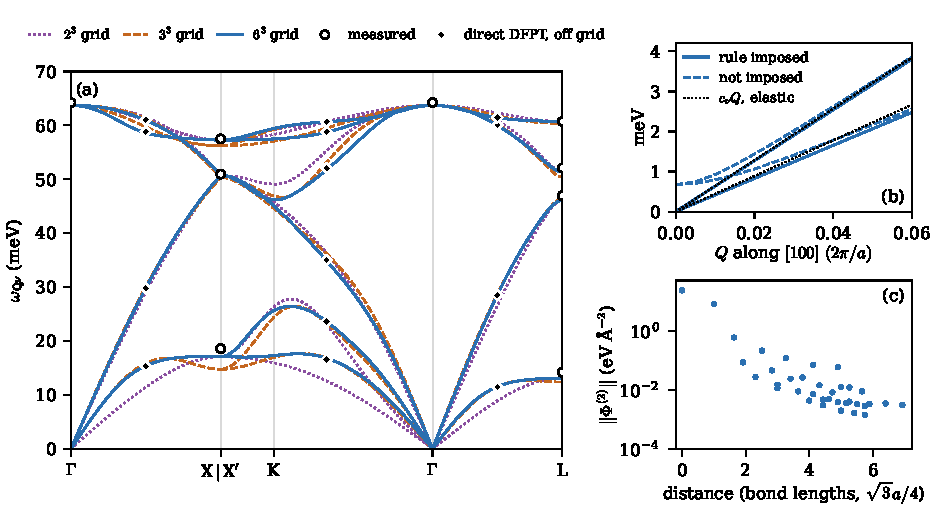
\includegraphics[width=\linewidth]{figures/ch05/fig5_3.pdf}
  \caption{Fourier interpolation of the force constants of silicon. All curves come from one set of dynamical matrices: density-functional perturbation theory with the PBE functional, an SG15 norm-conserving pseudopotential, a \SI{60}{Ry} cutoff, a $12^3$ grid of crystal momenta, $a = \SI{5.431}{\angstrom}$ and the natural mass of silicon, computed on a $6^3$ grid of wavevectors (the calculation of \cref{fig:5-si}). (a) Dispersion interpolated from the full $6^3$ grid (solid), from its $3^3$ subgrid (dashed) and from its $2^3$ subgrid (dotted), which contains only $\mathrm{\Gamma}$, X and L; acoustic sum rule imposed in each. Diamonds: frequencies from direct calculations, with the same settings, at three wavevectors that lie on none of the grids, $(0,0,\tfrac12)$, $(\tfrac12,\tfrac12,0)$ and $(\tfrac14,\tfrac14,\tfrac14)$ in units of $2\pi/a$. Circles: frequencies measured by inelastic neutron scattering at room temperature~\cite{dolling1963inelastic,nilsson1972study}, as tabulated in Ref.~\cite[Table~I]{savrasov1996linear}. (b) Acoustic branches along $[100]$ near $\mathrm{\Gamma}$ from the $6^3$ grid, with the sum rule imposed (solid) and not imposed (dashed); dotted, $\omega = c_\nu Q$ with the measured sound speeds \SI{8.43}{km.s^{-1}} (longitudinal) and \SI{5.84}{km.s^{-1}} (transverse). (c) Norm of the $3\times3$ blocks $\Phi^{(2),\alpha\beta}_{\kappa\kappa'}(\vect{0},\vect{R})$ of the $6^3$ grid against the distance $|\vect{R} + \vect{\tau}_{\kappa'} - \vect{\tau}_\kappa|$. The distance is that of the shortest image in the supercell, in units of the bond length $\sqrt3a/4 = \SI{2.35}{\angstrom}$.}
  \label{fig:5-dfpt}
\end{figure}

\Cref{fig:5-dfpt} tests this on silicon, with grids cut out of the single $6^3$ calculation of \cref{fig:5-si}. The $2^3$ grid has three inequivalent points, $\mathrm{\Gamma}$, X and L. At those points its frequencies agree with the $6^3$ ones to the last digit, \SI{17.06}{meV} for the transverse acoustic mode at X, as exactness on the grid requires. Between them it fails: at the three test points off all grids, its frequencies differ from direct DFPT by up to \SI{4.0}{meV}, a quarter of the transverse acoustic frequency. The $3^3$ grid, with four inequivalent points, misses X and puts the transverse acoustic mode there \SI{14}{\percent} low, at \SI{14.75}{meV}; at the test points, however, it is within \SI{1.2}{meV}. The $6^3$ grid reproduces them to \SI{0.3}{meV}, \SI{1.5}{\percent} at worst, which is below the \SI{2.6}{\percent} mean difference between this functional and experiment (\cref{sec:5.2}). Panel (c) shows why. The on-site block is \SI{23.3}{eV.\angstrom^{-2}} and the nearest-neighbor block \SI{8.0}{eV.\angstrom^{-2}}. Beyond the second neighbors most blocks fall below \SI{0.1}{eV.\angstrom^{-2}}, with one family of exceptions: the neighbors along the $\langle110\rangle$ zigzag chains of bonds, \SI{0.59}{eV.\angstrom^{-2}} at $a/\sqrt2 = \SI{3.84}{\angstrom}$, \SI{0.21}{eV.\angstrom^{-2}} at $\sqrt{19}\,a/4 = \SI{5.92}{\angstrom}$ and still \SI{0.12}{eV.\angstrom^{-2}} at $\sqrt2a = \SI{7.68}{\angstrom}$, \SI{1.5}{\percent} of the nearest-neighbor value at more than three bond lengths. These long-range constants along $\langle110\rangle$ are a known feature of the diamond and zincblende structures~\cite[Sect.~V.A.1]{baroni2001phonons}, and they are what the $2^3$ and $3^3$ supercells cannot hold. They control the flat transverse acoustic branch, which is where the coarse grids fail most.

The acoustic sum rule \cref{eq:5.2-asr} is exact for $E^{\mathrm{ad}}$ but not for its computed approximation. The violation comes chiefly from the exchange--correlation energy, which is integrated on a real-space grid that is fixed in space. A rigid translation of the crystal relative to the grid changes the energy by a small periodic amount, and the computed $\sum_{\vect{R}\kappa'}\Phi^{(2)}_{\kappa\kappa'}(\vect{0},\vect{R})$ is a small matrix $\Delta^{\mathrm{ASR}}_\kappa$ instead of zero. At $\vect{Q} = 0$ the acoustic modes then have $\omega^2 \sim \Delta^{\mathrm{ASR}}_\kappa/M_\kappa$ instead of zero, \SI{0.675}{meV} (\SI{0.163}{THz}) in \cref{fig:5-dfpt}(b). The simplest repair subtracts the violation from the on-site constants,
\begin{equation}
  \Phi^{(2),\alpha\beta}_{\kappa\kappa}(\vect{0},\vect{0}) \;\to\; \Phi^{(2),\alpha\beta}_{\kappa\kappa}(\vect{0},\vect{0}) - \sum_{\vect{R}\kappa'}\Phi^{(2),\alpha\beta}_{\kappa\kappa'}(\vect{0},\vect{R}) ,
  \label{eq:5.4-asrfix}
\end{equation}
after which \cref{eq:5.2-asr} holds exactly. The repair is not unique. When $\Delta^{\mathrm{ASR}}_\kappa$ is not symmetric in $\alpha\beta$, \cref{eq:5.4-asrfix} breaks the pair symmetry of \cref{sec:5.2}. Codes therefore also offer the smallest change of all the constants that restores both rules; in silicon $\Delta^{\mathrm{ASR}}_\kappa$ is a multiple of the identity by the cubic site symmetry, and the on-site repair keeps it. Neither repair imposes the rotational invariance of \cref{sec:5.2}.

The repair matters most where dark matter looks. Near $\mathrm{\Gamma}$ the unrepaired branches follow $\omega^2 \approx \omega_{\mathrm{ASR}}^2 + c_\nu^2Q^2$, with $\omega_{\mathrm{ASR}} = \SI{0.675}{meV}$, and they meet the straight lines only for $\omega \gg \omega_{\mathrm{ASR}}$. At $Q = 0.02\,(2\pi/a)$ the transverse acoustic frequency is \SI{1.07}{meV} instead of \SI{0.83}{meV}, \SI{29}{\percent} high; at $Q = 0.1\,(2\pi/a)$ the difference has dropped to \SI{1}{\percent}. With the rule imposed, the slopes along $[100]$ are 5.44 and \SI{8.34}{km.s^{-1}}, the PBE sound speeds of \cref{sec:5.2}. An acoustic-phonon search with a meV threshold samples exactly the region that the unrepaired constants get wrong (\cref{sec:9.2}). The size of $\omega_{\mathrm{ASR}}$ before the repair is also a cheap diagnostic of the real-space grid, which \cref{app:E.4} uses.
